% Készítette: Hajnal Máté
% Az Elte Programtervező Informatikus szakához tartozó Programozás tantárgyhoz tartozó házi feladatom.
% A feladatok közül a 11-es

\documentclass[12pt,a4paper]{article}			%Article dokumentum
\usepackage[utf8]{inputenc}						%UTF-8-as kódolás
\usepackage{t1enc}								%Furcsa betűk
\usepackage{fancyhdr}							%For footer and header

%LANGUAGE-FONT
%texlive-lang-hungarian package should be installed!
\usepackage[english,magyar]{babel}				%Magyar nyelv 
\usepackage{mathptmx}							%Times New Roman font
\usepackage[shortlabels]{enumitem}							%For enumerations
\usepackage{url}								%For URL-s
\usepackage[headheight=56pt]{geometry}			%For the heading gap

%MATHEMATICAL EXPRESSIONS
\usepackage[fleqn]{amsmath}						%Mathematical expressions
\usepackage{amsfonts}							%Mathematical fonts
\usepackage{bm}									%Bolding

%TABLES, TABULATING, DRAWING
\usepackage{array}
\usepackage{tabu}
\usepackage{multirow}
\usepackage{tabularx}
\usepackage{tikz}
\usepackage{stuki}

%HEADER
\sloppy
\fancyhead{}
\fancyhead[C]{\textbf{1.beadandó feladat/11.feladat}}
\fancyhead[R]{\today}
\fancyhead[L]{Hajnal~Máté \newline RJBSCJ \newline \url{hajnalmt@inf.elte.hu} \newline 5.csoport}
\pagestyle{fancy}

%Fejezet stílus deklaráció
\newcommand{\fejezet}[1]{\noindent \textbf{\textit{\large #1 \vspace{5mm}}}}

%DOCUMENT
\begin{document}
	\pagenumbering{arabic}
	
	%% Feladat fejezet %%
	\fejezet{Feladat}\\
	\textit{Egy határállomáson feljegyezték az átlépő utasok útlevélszámát. Melyik útlevélszámú
	utas fordult meg leghamarabb másodszor a határon?}
	\vspace{5mm}

	%% Specifikáció fejezet %%
	\fejezet{Specifikáció}\\
	Az értékeket egy tömbben tároljuk.
		% A feladat definiálása, Adathalmaz, Előfeltétel, Utófeltétel %
		\begin{flalign*}
			&A=(t:String^n,~min:\mathbb{N},~ind:\mathbb{N},~l:\mathbb{L})\\
			&Ef=(t=t')\\
			&Uf=(Ef~\wedge~min, ind, l = \min _{i=1, Vanmasodik() = igaz}^{i=n-1}(Vanmasodik()))
		\end{flalign*}
	
	%% Algoritmus fejezet %%
	\fejezet{Algoritmus}\\
	A feladatot a feltételes maximumkeresés tételére vezetjük vissza, csak esetünkben minimumkereséssel. \\
		% Megfeleltetés%
		\noindent\hfill
		\begin{stukibox}[6cm]
			\stm*{\bfseries{felt. max. ker.}}
			\stm*[4]{i:m..n $\sim$ 1..n-1 \\ $\beta(i) \sim$ Vanmasodik()=igaz \\ f(i) $\sim$ Vanmasodik()}
		\end{stukibox}
		\hfill
		\begin{stukibox}[4cm]
			\stm*{\bfseries{pessz. lin. ker.}}
			\stm*[4]{j:m..n $\sim$ i+1..n \\ $ \beta(i) \sim$ t[i] = t[j] }
		\end{stukibox}
		\hfill{}

		\noindent\hfill
		\begin{stuki}[\textwidth]
			\stm*{l, min, ind:=hamis, n, 0}
			\begin{WHILE}{4}{\stm{i=0..n-1}}
				\stm{j,l_2=Vanmasodik()}
				\begin{CASE}[1]{2}{6}
				\WHEN[1] {\stm[1]{\lnot l_2 }}
					\stm*[1]{SKIP}
				\WHEN[3] {\stm[1]{l_2 \land l}}
					\begin{IF}{1}{\stm{min>j}}
						\stm{min,ind=j,i}
					\ELSE
						\stm*{SKIP}
					\end{IF}
				\WHEN[2] {\stm[1]{l_2 \land \lnot l}}
					\stm[1]{l, min, ind = igaz, j, i}
				\end{CASE}
			\end{WHILE}
		\end{stuki}
		\begin{stuki*}{Vanmasodik} 
			\stm{l_2, j:= hamis, i}
			\begin{WHILE}{2}{\stm{k=i+1..n}}
				\begin{IF}{1}{\stm{t[i]=t[k] \land \lnot l_2}}
					\stm{l_{2}, j := igaz, k}
				\ELSE
					\stm{SKIP}
				\end{IF}
			\end{WHILE}
		\end{stuki*}
		\vspace{5mm} 
	
	%% Implementáció fejezet %%
	\fejezet{Implementáció}\\
		% Adattípusok %
		{\large Adattípusok megvalósítása} \vspace{2mm} \\
		A kódoláskor a t tömböt \texttt{vector<int>}-ként deklaráltam, amelynek mérete \texttt{t.size()} alakban érhető el. Mivel a vektor C++-ban 0-tól indexelődik, így a tervbeli 2-től n-1-ig tartó ciklus az esetünkben \texttt{1-től t.size()-2-ig} fog tartani. A struktogramm kódja így:
		% A struktogramm %
		\texttt{
			\begin{tabbing}
				\hspace{2cm}\= l=false \+\\
				for (int i=1; i < t.size()-1; ++i) \{\\
				\hspace{1cm}\= if (t[i-1] > t[i] \&\& t[i+1] > t[i] \&\& l) \{ \+\\
					\hspace{1cm}\=if (t[i] > max) \{ \+\\
					\hspace{1cm}\=max = t[i]; \+\\
					ind = i+1;\-\\
					\}\-\\
				\}\\
				else if (t[i-1] > t[i] \&\& t[i+1] > t[i]) \{ \+\\
					l = true;\\
					max = t[i];\\
					ind = i+1;\-\\
				\} \-\\
			\}
			\end{tabbing}
		}
		% Bemenő adattípusok %
		\noindent {\large Bemenő adatok formája} \vspace{2mm}\\
		A bemenő adatokat egy szöveges állományból kell a tömbbe bemásolni. Az állományban a megadott neveket szóközökkel, tabulátor jelekkel vagy sorvége jelekkel elválasztva kell beírni. Az állomány minden sorát sorvége jel zárja le. Például:
		% Bemenő adatokra példa %
		\texttt{
			\begin{tabbing}
			\hspace{2cm}\= 12 6 8 11\+\\
			45 \hspace{1cm} 78\\
			44 324\-
			\end{tabbing}
		}\vspace{2mm}
		% Függvények kapcsolódása %
		\noindent {\large A függvények kapcsolódási szerkezete} \vspace{2mm}\\
		A kódban több függvényt is használunk. Az \texttt{Maxvolgy()} tartalmazza a tervben leírt keresést, a \texttt{ReadFromFile()} tölti fel egy szöveges állományból a tömböt nevekkel, ezeket a függvényeket pedig a \texttt{main()} hívja, amelyik az eredmény kiírását is végzi.
		% A függvény kapcsolódást szemléltető ábra %
		\begin{center}
		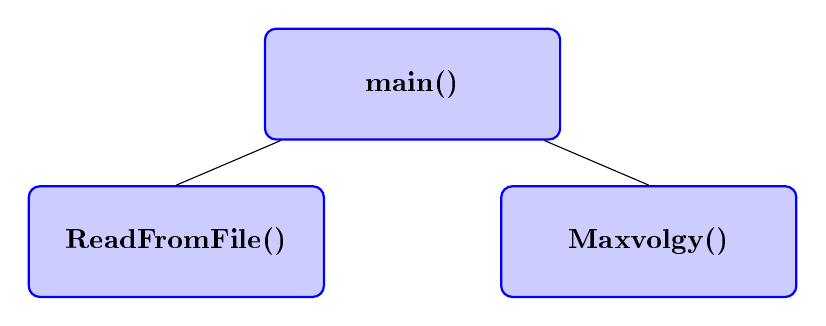
\begin{tikzpicture}
			[level distance=20mm, sibling distance=60mm, align=center, block/.style ={rectangle, draw=blue, thick, fill=blue!20,text width=10em,align=center, rounded corners, minimum height=4em}];
			\node [block] (main) {\textbf{main()}}
				[child anchor=north]
				child {node [block] (readfromfile) {\textbf{ReadFromFile()}}}
				child {node [block] (maxvolgy) {\textbf{Maxvolgy()}}};
		\end{tikzpicture}\vspace{2mm}\\
		\end{center}

	%% Tesztelés fejezet %%
	\fejezet{Tesztelési terv}\\
		% Fekete doboz esetek %
		\renewcommand{\labelenumi}{\Alph{enumi}.}
		\renewcommand{\labelenumii}{\arabic{enumii}.}
		{\large A feladat specifikációjára épülő (fekete doboz) tesztesetek} \vspace{2mm}\\
		Érvényes tesztesetek (most érvénytelen bemenet nem lehet):
		\begin{enumerate}		
			\item \textbf{Maximum keresés} tesztesetei:\\
			\textbf{intervallum hossza} szerint
			\begin{enumerate}
				\item \textit{nulla} hosszú: 
				\begin{itemize}[label={}]
					\item Egyetlen érték sincs (üres vagy csak elválasztójelekből álló fájl)\\
					(t1.txt: [] - válasz hamis)\\
					(t2.txt: [    ] - válasz hamis)
				\end{itemize}
				\item \textit{egy} hosszú
				\begin{itemize}[label={}]
					\item Egyetlen érték van ami pozitív\\
					(t3.txt: [4] - válasz hamis)
					\item Egyetlen érték van ami 0\\
					(t4.txt: [0] - válasz hamis)
					\item Egyetlen érték van ami negatív\\
					(t5.txt: [-6] - válasz hamis)
				\end{itemize}
				\item \textit{kettő} hosszú
				\begin{itemize}[label={}]
					\item Két egész érték\\
					(t6.txt: [-5 6] - válasz hamis)
				\end{itemize}
				\item \textit{három} hosszú
				\begin{itemize}[label={}]
					\item Nincs völgy a sorozatban\\
					(t7.txt: [1 2 3] - válasz hamis)
					\item Van völgy a sorozatban\\
					(t8.txt: [3 2 3] válasz: igaz, 2. index, 2 értékkel)
				\end{itemize}
			\end{enumerate}
			\textbf{völgyek száma} szerint
				\begin{enumerate}
					\item Nincs elég elem a tömbben, hogy völgy legyen\\
					(t6.txt: [-5 6] - válasz hamis)
					\item Van elég elem a tömbben, hogy lehessen völgy de még sincsen\\
					(t7.txt: [1 2 3] - válasz hamis)
					\item Egy völgy van a sorozatban az a maximum\\
					(t8.txt: [3 2 3] válasz: igaz, 2. index, 2 értékkel)
					\item Több völgy van a sorozatban, az első a maximum\\
					(t9.txt: [15 6 5 12 4] válasz: igaz, 3. index, 5 értékkel)
					\item Több völgy van a sorozatban, nem az első a maximum\\
					(t10.txt: [15 6 45 12 42] válasz: igaz, 4. index, 12 értékkel)
				\end{enumerate}
			\item \textbf{Különleges} esetek
				\begin{enumerate}
					\item Negatív számok (nincs különbség beolvasásban)
					\item Betűket tartalmazó input beolvasása (A karakterek ASCII kódja kerül beolvasásra számként)
					\item Nem érvényes teszteset, ha a signed integer érték maximumánál $2^{31}-1=2147483657$-nél nagyobb vagy a minimumánál $-2^{31}=-21474836578$-nál kisebb értéket tartalmaz a teszt.
				\end{enumerate} 
		\end{enumerate}

		% Fehér doboz esetek %
		\renewcommand{\labelenumi}{\arabic{enumi}.}
		\noindent{\large A megoldó programra épülő (fehér doboz) tesztesek} \vspace{2mm}
		\setlist[enumerate,1]{leftmargin=2cm}
		\begin{enumerate}[1, itemsep=0ex]
			\item Hibás vagy nem létező állománynév megadása.
			\item Állomány nevének megadása parancssorból
			\item Ismételt futtatás kipróbálása
			\item Olyan állomány olvasása, ahol egy sorban több érték is található egyetlen illetvetöbb szóközzel és/vagy tabulátor jellel elválasztva (t12.txt).
			\item Olyan állomány olvasása, ahol minden érték külön sorban van. (t11.txt).
			\item Főprogram ciklusának ellenőrzése: olyan bemenő adatokkal, amelyekre a ciklus egyszer sem fut le (Pl: t1.txt), pontosan egyszer fut le (Pl: t7.txt), többször lefut és igaz logikai értékkel lép ki (Pl: t9.txt), vagy hamis logikai értékkel lép ki (Pl: t13.txt).
		\end{enumerate}
\end{document}
